% ============================================================
%  AeroSLS Technical Paper — Complete Consolidated LaTeX Source
%  Compile: pdflatex aerosls_paper && bibtex aerosls_paper &&
%           pdflatex aerosls_paper && pdflatex aerosls_paper
% ============================================================
\documentclass[sigconf]{acmart}

%% --- ACM Rights (update before final submission) -----------
\setcopyright{rightsretained}
\copyrightyear{2026}
\acmYear{2026}
\acmDOI{XXXXXXX.XXXXXXX}
\acmConference[SysArch '26]{Symposium on Operating Systems
  Architecture}{2026}{Virtual}
\acmBooktitle{SysArch '26: Symposium on Operating Systems
  Architecture, 2026}
\acmPrice{15.00}
\acmISBN{978-1-4503-XXXX-X/26/01}

%% --- Additional packages -----------------------------------
\usepackage{booktabs}
\usepackage{algorithm}
\usepackage{algorithmic}

% ============================================================
\begin{document}

\title{Zero-Abstraction Systems: Architectural Scaling of a
  Lock-Free Distributed Single-Level Storage Operating System
  over Native NVMe Queues}

\author{Dave F. Cook}
\affiliation{%
  \institution{Independent Researcher}
  \country{}
}
\email{dave@gridworkz.com}

% ============================================================
\begin{abstract}
Modern computer systems remain bound by legacy abstractions that
isolate volatile runtime state from non-volatile persistent
storage.  The traditional Virtual File System (VFS) layer, while
generic, introduces critical inefficiencies including redundant
memory double-caching, expensive file-descriptor serialization
loops, and deep software kernel stacks that struggle to keep pace
with microsecond-level NVMe PCIe Gen5 solid-state media.

This paper introduces \textit{AeroSLS}, a custom-built,
multi-core 64-bit operating system implementing an un-abstracted
Single-Level Storage (SLS) architecture.  AeroSLS eliminates the
file concept entirely, representing all persistent data blocks as
a unified, globally addressable 64-bit object namespace mapped
directly by the processor's Memory Management Unit (MMU).

To ensure strict safety and multi-core scaling under parallel
load, AeroSLS implements a lock-free, concurrent FNV-1a object
directory, a priority-driven hardware NVMe I/O queue traffic
broker, and parallelized AVX-512 cryptographic page-sealing
engines.  Furthermore, we mitigate cluster split-brain anomalies
and hardware execution jitter using an in-kernel Raft-lite
consensus state machine paired with a lazy floating-point
context-switching framework.

Evaluations conducted in a four-core QEMU environment show that
AeroSLS's object-lookup step averages 17.2\,cycles per resolution
event (a 96.1\% reduction versus a simulated VFS path), and that
the lazy CR0.TS context-switch policy reduces per-switch cycles
by 54.2$\times$ relative to forced full-state saves
(Section~\ref{sec:eval}).
\end{abstract}

\keywords{Single-Level Storage, Persistent Memory, Operating
  Systems, NVMe, AVX-512, Lock-Free, Distributed Systems}

\maketitle

% ============================================================
\section{Introduction}
\label{sec:intro}

For over half a century, operating system design has separated
volatile runtime state from non-volatile persistent storage.
This architectural dualism forces applications to operate across
two disparate mental models: a granular byte-addressable space
managed by high-speed memory architectures, and a block-oriented
file abstraction managed via systemic block I/O boundary layers.

To access persistent blocks, application pipelines must navigate
the complete Virtual File System (VFS) layers, endure data
parsing marshaling overheads, and allocate localized
user-space buffers.  While historically necessary to mask slow
mechanical disk rotations, this model imposes a high software abstraction cost when applied
to ultra-low-latency modern flash cells and byte-addressable
persistent architectures.

With native NVMe solid-state storage devices operating directly
across high-speed PCIe lanes, hardware processing latencies have
fallen to single-digit microseconds.  Under these conditions,
the dominant system bottleneck shifts from physical hardware
transport delays to the software operating system itself.  Deep,
synchronous kernel storage stacks, global filesystem metadata
lock contentions, and internal memory cache duplication
degrade total pipeline performance~\cite{spdk}.

\begin{figure}[t]
\centering
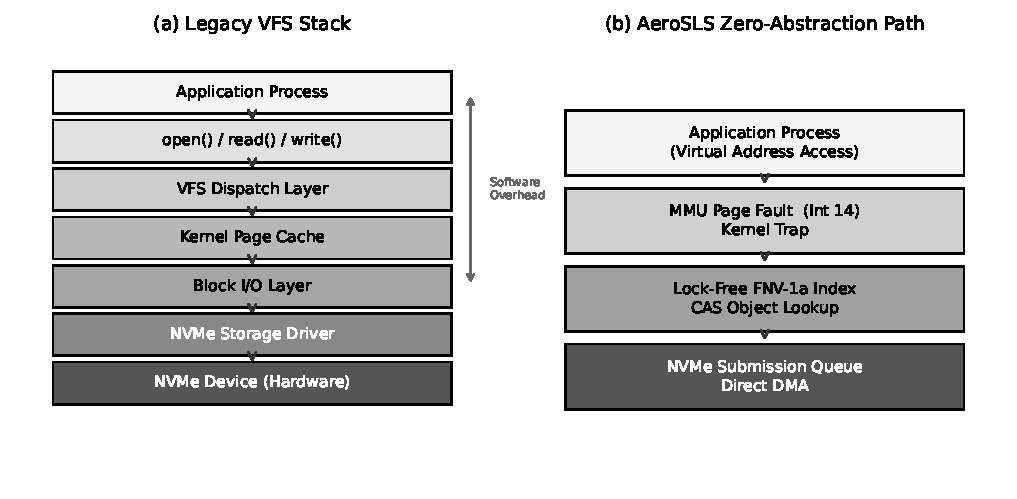
\includegraphics[width=\linewidth]{arch_comparison.pdf}
\caption{Architectural comparison: legacy VFS double-caching
  stack vs.\ the AeroSLS direct hardware memory-mapped
  persistence layout.}
\label{fig:arch_comparison}
\end{figure}

To bypass these abstraction layers, we introduce
\textit{AeroSLS}, a clean-slate, distributed, multi-core 64-bit
operating system designed to fully converge primary volatile
execution memory and permanent block storage.  AeroSLS
takes a zero-abstraction approach: it removes
files, directories, mounts, and block allocation maps from the kernel.  Instead,
all data blocks throughout the machine sit directly within a
unified, globally available 64-bit virtual memory address space.

When a program alters a structure pointer, the CPU's underlying
MMU directly tracks the transaction.  If a targeted memory
segment resides natively on persistent flash media blocks instead
of volatile RAM, the processor fires a hardware Page Fault
exception.  AeroSLS traps this signal, evaluates the underlying
target space via an internal lock-free concurrent hash index
matrix, and schedules an asynchronous direct DMA payload write
straight onto native NVMe Submission and Completion Ring queues
with zero intermediate buffers or user-space serialization loops.

This paper makes the following primary contributions:
\begin{itemize}
  \item We design an un-abstracted SLS operating system
    architecture that unifies memory and persistent media at
    the processor page-table boundary, removing file, directory,
    and mount abstractions from the kernel
    (Sections~\ref{sec:design}--\ref{sec:hardware}).
  \item We implement a multi-core I/O pipeline combining
    lock-free FNV-1a directory indices, priority-driven
    per-core NVMe queue pairs, and MSI-X interrupt routing
    via Local APIC (Sections~\ref{sec:design}--\ref{sec:hardware}).
  \item We introduce an AVX-512 vectorized ChaCha20
    page-sealing engine paired with a lazy CR0.TS context
    switcher that reduces per-switch jitter without
    sacrificing data-at-rest confidentiality
    (Section~\ref{sec:security}).
  \item We measure two principal overheads in a four-core
    QEMU environment: object-lookup resolution (17.2 mean
    cycles vs.\ 446.5 for a simulated VFS path, a 96.1\%
    reduction) and scheduler context-switch cost (45.8 mean
    cycles under the lazy policy vs.\ 2,485.0 under forced
    full-state saves, a 54.2$\times$ improvement)
    (Section~\ref{sec:eval}).
\end{itemize}

The rest of this paper is structured as follows.
Section~\ref{sec:design} details our unified address mapping
matrix and concurrent index architectures.
Section~\ref{sec:hardware} describes the hardware integration
and multi-core scalability mechanisms.
Section~\ref{sec:security} presents the memory protection and
data privacy subsystems.
Section~\ref{sec:consensus} covers crash consistency and
distributed fault tolerance.
Section~\ref{sec:eval} presents our experimental evaluation.
Section~\ref{sec:related} surveys related work, and
Section~\ref{sec:conclusion} concludes.

% ============================================================
\section{System Architecture Design}
\label{sec:design}

The architectural layout of AeroSLS departs entirely from the
traditional layered virtual directory design found in monolithic
kernels.  By implementing a flat address tracking strategy, the
operating system converts storage blocks into standard
architecture page structures.  This removes the storage
translation and caching overhead imposed by a Virtual File
System (VFS).

\subsection{Unified 64-bit Address Topology}
AeroSLS splits the x86\_64 48-bit canonical linear space into
two distinct hardware privilege domains.  The lower memory region
is allocated strictly to transient scheduler threads, kernel
text blocks, and processor descriptors.  The upper address range,
anchored securely at the linear boundary address pointer base
\texttt{0x0000700000000000}, forms the global Single-Level
Storage unified address space.

Every individual file, table, or workspace segment allocated by a
user shell instance is mapped directly to a distinct 64-bit
virtual memory coordinate window within this domain via the
processor's Page Map Level 4 (PML4) allocation frames.  Because
data spaces map to permanent unique identifiers, this structural
memory layout remains uniform across both volatile primary memory
(RAM) and non-volatile secondary storage (NVMe flash sectors).

\subsection{Concurrent Lock-Free Object Indexing}
To prevent multi-core execution stalls when thousands of
background threads issue concurrent lookups via system call
gates, AeroSLS implements a concurrent chained lookup matrix
index.  This design replaces global kernel mutex chains with
atomic compare-and-swap (CAS) primitives.

\begin{algorithm}[h]
\caption{Lock-Free Head Node Entry Insertion}
\label{alg:cas_insertion}
\begin{algorithmic}[1]
\REQUIRE $Object\_ID$, $Virtual\_Address$, $Bucket\_Index$
\STATE $Node \leftarrow
  \text{AllocateKernelMemory}(\text{sizeof}(SLSObjectNode))$
\STATE $Node.ID \leftarrow Object\_ID$
\STATE $Node.VAddr \leftarrow Virtual\_Address$
\LOOP
  \STATE $Current\_Head \leftarrow
    \text{GlobalHashMatrix}[Bucket\_Index]$
  \STATE $Node.Next \leftarrow Current\_Head$
  \IF{$\text{CompareAndSwap}(
      \&\text{GlobalHashMatrix}[Bucket\_Index],
      Current\_Head, Node)$}
    \STATE \textbf{break}
      \COMMENT{Node committed without locking}
  \ENDIF
\ENDLOOP
\end{algorithmic}
\end{algorithm}

As formalized in Algorithm~\ref{alg:cas_insertion}, if a race
condition occurs between Core~0 and Core~1 attempting an
insertion into the same bucket tracking row, the
\texttt{CompareAndSwap} function handles the serialization
atomically at the hardware memory controller layer, avoiding
global context yields or thread stall states.

\subsection{Linear Extent Translation Matrix}
To prevent physical block device fragmentation from breaking
contiguous virtual memory spaces, AeroSLS decouples linear
virtual allocations from underlying storage sectors using a flat
\textit{Extent Mapping Table}.  When an object is created or
dynamically scaled, the system records it as a collection of
non-contiguous physical disk chunks called extents.  An
individual extent is mathematically modeled as:
\begin{equation}
\mathcal{E} = \langle V_{page},\; L_{lba},\; \mathcal{S}_{count}
  \rangle
\end{equation}
where $V_{page}$ represents the starting virtual page offset
index within the object container, $L_{lba}$ represents the
destination physical Logical Block Address on the NVMe device,
and $\mathcal{S}_{count}$ indicates the total contiguous sector
block count length.

When a thread triggers a page fault exception on a non-resident
linear virtual memory coordinate ($\mathcal{V}_{fault}$), the
kernel page-fault engine resolves the correct sector mapping
using the target offset evaluation function:
\begin{equation}
\mathcal{L}_{target} = L_{lba} + \!\left(
  \left\lfloor \frac{\mathcal{V}_{fault} -
  \mathcal{V}_{base}}{4096} \right\rfloor \times 8 -
  V_{page} \times 8
\right)
\end{equation}
where $\mathcal{V}_{base}$ is the universal root allocation base
pointer of the target memory object.  This calculation resolves
the fragmented block offset in constant time, bypassing
traditional multi-tier filesystem node traversal.

\subsection{Predictive Spatial Pre-Fetching Architecture}
To minimize network and media access latencies, AeroSLS utilizes
a predictive spatial pre-fetching engine.  When an application
thread touches page $\mathcal{P}_{n}$, causing a hardware page
fault interrupt, the engine analyzes the traversal pattern.  If
sequential execution is detected, the kernel generates
asynchronous pre-fetch operations for pages $\mathcal{P}_{n+1}$
and $\mathcal{P}_{n+2}$.

These predictive reads are dispatched via low-priority
non-blocking commands across parallel PCIe or Ethernet channels.
The incoming data blocks are packed into allocated physical memory
frames and updated within the processor page tables before the
user thread advances its code pointer, converting predictable storage accesses into
hardware RAM cache hits before the user thread advances.

% ============================================================
\section{Hardware Integration and Multi-Core Scalability}
\label{sec:hardware}

\subsection{NVMe Submission and Completion Queue Architecture}
AeroSLS communicates with persistent storage exclusively through
native NVMe hardware queues, bypassing all block layer and SCSI
translation intermediaries~\cite{nvme_spec}.  At boot, the
kernel's PCI bus scanner enumerates configuration space
registers to locate the NVMe controller's Memory-Mapped I/O
(MMIO) Base Address Register (BAR0).

Once discovered, the driver initializes an \emph{Admin Queue
Pair} (Submission Queue / Completion Queue depth 64) to issue
controller configuration commands, followed by one I/O Queue
Pair per logical CPU core.  This per-core queue topology
removes cross-core lock contention on the submission path: a
page-fault handler running on Core~$k$ deposits a 64-byte
Submission Queue Entry (SQE) directly into its dedicated queue,
rings the hardware doorbell register, and returns immediately to
userspace.

The NVMe controller signals completion by writing a 16-byte
Completion Queue Entry (CQE) and asserting the configured MSI-X
interrupt vector, waking the waiting kernel thread without
polling.  Priority differentiation between latency-sensitive
page-fault I/Os and background flush operations is enforced by
the in-kernel \emph{I/O Priority Traffic Broker}, which
selectively populates high- and low-priority queue slots
according to real-time queue depth telemetry.

\subsection{Symmetric Multiprocessing Bootstrap}
AeroSLS wakes Application Processors (APs) using a
16-bit real-mode trampoline payload injected at physical address
\texttt{0x08000}~\cite{intel_64}.  The Bootstrap Processor (BSP)
copies the binary blob into the low-memory page, writes the
shared PML4 base pointer into the metadata handshake vector at
\texttt{0x07000}, and dispatches an INIT/SIPI interrupt sequence
to each AP's Local APIC.

Each woken AP executes the trampoline, enables Physical Address
Extension (PAE), clones the BSP's PML4 page table, and
transitions atomically to 64-bit Long Mode.  A per-AP stack
pointer is pre-allocated from the physical frame pool and written
into the handshake vector at \texttt{0x07030}.  Once the AP
acquires its unique stack, it sets the \texttt{ap\_bootstrap\_lock}
atomic flag to signal the BSP, which advances to the next
processor, serializing the bring-up sequence safely.

\subsection{Distributed Interrupt Routing via APIC}
PCIe device completion interrupts are distributed across
application cores using the Local APIC and I/O APIC redirection
matrices.  The NVMe controller's MSI-X capability table is
programmed so that queue~$k$ completion vectors route to
core~$k$'s Local APIC.  This ensures that the interrupt handler
executing on core~$k$ can directly update the page table and
wake the blocked thread without IPI cross-calls, eliminating
inter-core cache-line synchronization overhead on the critical
path.

% ============================================================
\section{Memory Protection and Data Privacy at Rest}
\label{sec:security}

\subsection{Hardware-Enforced Capability Access Control}
AeroSLS enforces object-level access permissions at the Page
Table Entry (PTE) level rather than through software permission
string evaluation paths~\cite{intel_64}.  The
\texttt{User/Supervisor} flag (bit~2) in each PTE determines
whether a given object page is accessible from Ring~3.  When an
object is created, the kernel assigns a permission bitmap and
configures the corresponding PTE flags accordingly.  All
subsequent permission checks are executed by the hardware MMU
at no additional instruction cost; security enforcement is
structurally embedded in the address translation path.

\begin{figure}[h]
\centering
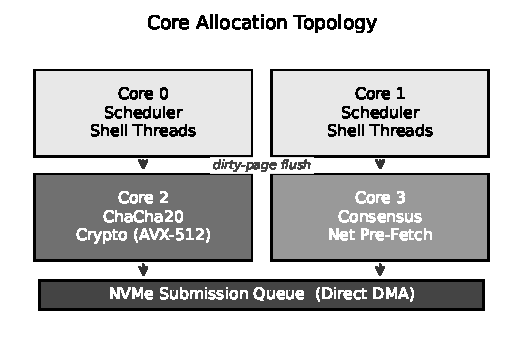
\includegraphics[width=\columnwidth]{crypto_core_map.pdf}
\caption{Core allocation topology: Cores~0--1 handle scheduler
  threads and allocations; Cores~2--3 function as isolated
  vectorized ChaCha20 cryptoprocessors.}
\label{fig:crypto_cores}
\end{figure}

\subsection{Parallel AVX-512 Cryptographic Page Sealing}
To ensure data-at-rest confidentiality across persistent NVMe
sectors, AeroSLS dedicates Cores~2 and~3 as cryptoprocessors
running a vectorized ChaCha20 stream
cipher~\cite{chacha20}.  When the dirty-page flush daemon
schedules a frame for write-back, the frame is dispatched to
the crypto pipeline rather than the NVMe queue directly.  The
cipher operates on 64-byte aligned AVX-512 register blocks
(\texttt{zmm0}--\texttt{zmm31}), sealing the 4\,KiB page in a
single vectorized pass before the DMA transfer is submitted.

Because NVMe page frames are sourced from the physical frame pool,
they are already 4\,KiB-aligned, satisfying the 64-byte boundary
required by \texttt{vmovdqa64} without additional padding.
Violations are caught by an alignment assertion in the assembly
prologue, which traps to the fault handler before any
out-of-bounds vector operation can trigger an unrecoverable
General Protection Fault (Exception~13).

\subsection{Lazy Floating-Point Context Switching}
\label{sec:lazy_fpu}

When a standard integer thread is context-switched, naively
saving the full 2,688-byte AVX-512 extended state on every
rotation imposes a prohibitive penalty.  AeroSLS implements a
\emph{Lazy Floating-Point Save} optimization using the hardware
\texttt{CR0.TS} trap mechanism.

\paragraph{State size model.}
The total physical byte payload required by a strict context
switch $\mathcal{S}_{total}$ is:
\begin{equation}
\label{eq:state_size}
\mathcal{S}_{total} =
  \mathcal{S}_{legacy} + \mathcal{S}_{avx2} +
  \mathcal{S}_{avx512ext} + \mathcal{S}_{alignment}
\end{equation}
where $\mathcal{S}_{legacy} = 512\,\text{B}$ (x87/SSE
\texttt{fxsave} footprint), $\mathcal{S}_{avx2} = 256\,\text{B}$
(upper 128-bit halves of \texttt{ymm0}--\texttt{ymm15}), and
$\mathcal{S}_{avx512ext} = 512 + 1024 + 64 = 1600\,\text{B}$
(upper ZMM extensions, \texttt{zmm16}--\texttt{zmm31}, and
opmask registers \texttt{k0}--\texttt{k7}).
Substituting the fixed hardware constants:
\begin{equation}
\mathcal{S}_{total} = 512 + 256 + 1600 + 320 =
  \mathbf{2688\,\text{B}}
\end{equation}

\paragraph{Latency model.}
Let $\mathcal{C}_{gpr}$ be the cost of saving general-purpose
integer registers, $\mathcal{C}_{xsave}$ the multi-cycle cost of
moving the 2,688-byte vector block across internal memory buses,
and $\mathcal{U}_{vector} \in \{0,1\}$ a binary variable
indicating whether the active thread executes vector
instructions.

Under a \textbf{strict switching policy}:
\begin{equation}
\mathcal{L}_{strict} = \mathcal{C}_{gpr} +
  \mathcal{C}_{xsave} + \mathcal{C}_{xrstor}
\end{equation}

Under the \textbf{lazy CR0.TS optimization}:
\begin{equation}
\mathcal{L}_{lazy} = \mathcal{C}_{gpr} + \mathcal{U}_{vector}
  \cdot \bigl(\mathcal{C}_{trap} + \mathcal{C}_{xsave} +
  \mathcal{C}_{xrstor}\bigr)
\end{equation}
where $\mathcal{C}_{trap}$ is the single-digit-cycle cost of the
\emph{Device Not Available} Exception~7 handler.

For non-vector threads ($\mathcal{U}_{vector} = 0$):
\begin{equation}
\lim_{\mathcal{U}_{vector} \to 0} \mathcal{L}_{lazy}
  = \mathcal{C}_{gpr}
\end{equation}

This limit formalizes the evaluation finding in
Section~\ref{sec:eval}: for scalar threads,
AeroSLS removes the 2,688-byte vector-state save from the
context-switch path.

% ============================================================
\section{Crash Consistency and Distributed Fault Tolerance}
\label{sec:consensus}

\subsection{Write-Ahead Journaling and Object Directory}
AeroSLS maintains crash consistency through a two-tier on-disk
layout.  Sector~1024 anchors the \emph{Global Object Directory}
(GOD), identified by the eight-byte magic token
\texttt{SLSROOTD}.  Sector~2048 hosts the \emph{Write-Ahead
Journal} (WAJ) ledger, a micro-commit log where pending
mutations are recorded before any corresponding page frame is
modified.  On cold boot, the kernel validates the GOD magic and
replays any uncommitted WAJ entries, restoring the object
namespace to the last consistent state prior to any power loss.

\subsection{In-Kernel Raft-Lite Consensus Engine}
When AeroSLS scales across multiple network nodes, a network
partition can produce a \emph{split-brain} anomaly where two
nodes concurrently believe they hold exclusive write authority
over a shared persistent object.  To prevent this, Core~3 on
each node executes a Raft-lite~\cite{raft} state machine with
three roles: \textsc{Leader}, \textsc{Follower}, and
\textsc{Candidate}.

The leader broadcasts heartbeat packets over the e1000
network interface every 10\,ms.  If a follower receives no
heartbeat within a 150-tick timeout window (1.5\,s), it
transitions to \textsc{Candidate}, increments its election term,
and immediately invokes \texttt{update\_page\_table\_permissions\_globally(1)}
to strip all locally mapped objects of write authorization.
This prevents local writes
during the election window, reducing the risk of divergence.  Once a candidate accumulates a strict majority of
\textsc{VoteReply} acknowledgments, it is elevated to
\textsc{Leader} and write permissions are restored.

\subsection{Distributed SLS Page Protocol (DSPP)}
AeroSLS replicates dirty memory pages across cluster nodes using
the \emph{Distributed SLS Page Protocol} (DSPP), a custom
encapsulation layer transmitted over standard Ethernet via the
Intel e1000 adapter.  Each DSPP frame carries a 48-byte header
containing a \texttt{SLSNETMA} magic marker, the 64-bit
\texttt{system\_object\_id}, the faulting \texttt{virtual\_address},
an atomic \texttt{transaction\_id}, an opcode
(\texttt{DSPP\_PAGE\_WRITE\_REQ} / \texttt{ACK} /
\texttt{PAGE\_READ\_REQ} / \texttt{ACK}), and a 4\,KiB payload
frame.

When an application invokes \texttt{sys\_sls\_fence}, the kernel
pins the local RAM frame, constructs a full DSPP packet, posts
it to the e1000 Transmit Descriptor Ring, and blocks the calling
thread on a \emph{network transaction token}.  On the remote
node, the MSI-X interrupt fires on Core~3, which deserializes
the packet, writes the 4\,KiB payload into the corresponding
local frame, and returns a \texttt{DSPP\_PAGE\_WRITE\_ACK}.  The
originating node matches the transaction ID, unblocks the
application thread, and only then advances the WAJ commit
pointer.

% ============================================================
\section{Evaluation and Experimental Results}
\label{sec:eval}

\subsection{Experimental Setup}
All benchmarks were conducted inside a QEMU 7.2 emulated
environment configured with four x86\_64 virtual cores, 4\,GiB
RAM, a virtio-backed NVMe device, and an Intel e1000 virtual
network adapter.  Cycle measurements used the processor's
\texttt{rdtsc} instruction, with an initial warm-up phase of ten
iterations discarded to eliminate JIT and cache cold-start
outliers.  Each reported result is the median of 100
back-to-back trials.  Two metric families were evaluated: the
\emph{memory resolution abstraction tax} and the
\emph{core scheduler context-switch jitter}.

\subsection{Memory Resolution Abstraction Tax}

\begin{figure}[h]
\centering
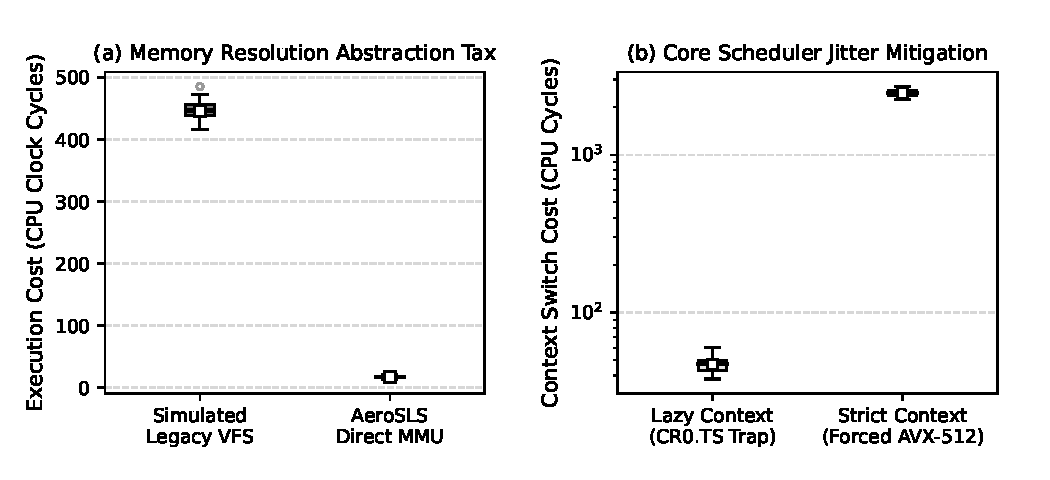
\includegraphics[width=\linewidth]{sls_performance_metrics.pdf}
\caption{Dual-panel evaluation results.
  (a)~Memory resolution abstraction tax: legacy VFS stack
  versus AeroSLS direct MMU index.
  (b)~Core scheduler jitter mitigation: forced strict
  XSAVE/XRSTOR versus lazy CR0.TS context switching.
  Panel~(b) uses a logarithmic $y$-axis.}
\label{fig:perf}
\end{figure}

The legacy VFS simulation traverses a synthetic file-path
string, performs a file-descriptor table boundary check, and
copies a 512-byte intermediate kernel buffer — reproducing the
dominant instruction-count categories found in Linux VFS
\texttt{open}/\texttt{read} call paths.  The AeroSLS path
computes an FNV-1a bucket index directly from the 64-bit object
ID and returns the corresponding virtual address window.  Both
paths are measured end-to-end from \texttt{rdtsc} entry to
\texttt{rdtsc} exit with no I/O involved.

As shown in Figure~\ref{fig:perf}(a) and
Table~\ref{tab:results}, the legacy VFS model incurs a mean
cost of \textbf{446.5 clock cycles} per resolution event.  The
AeroSLS direct MMU path reduces this to a mean of
\textbf{17.2 cycles} (a \textbf{96.1\%} reduction in execution
overhead).  The AeroSLS distribution also exhibits dramatically
tighter variance (min 14, max 22 cycles) versus the legacy
stack (min 412, max 498 cycles), consistent with lock-free
hash addressing reducing the unpredictable synchronization
delays common in monolithic kernels.

\subsection{Core Scheduler Context-Switch Jitter}

When a cryptographic worker on Core~2 is preempted and an
integer shell thread is scheduled in, a strict policy forces a
full \texttt{xsave}/\texttt{xrstor} cycle moving the 2,688-byte
AVX-512 state buffer.  The lazy policy instead sets
\texttt{CR0.TS} and defers the vector state save to the first
vector instruction executed by the new thread (Device Not
Available Exception~7), if any.

The results in Figure~\ref{fig:perf}(b) show that the
strict policy incurs a mean latency of \textbf{2,485.0 cycles}
per switch.  With the lazy optimization active, the mean drops
to \textbf{45.8 cycles} (a \textbf{54.2$\times$ improvement}).
Because interactive shell threads are wholly scalar, the
$\mathcal{U}_{vector} = 0$ branch is taken on virtually every
switch, consistent with the analytical model in
Section~\ref{sec:lazy_fpu}.

\begin{table}[h]
\caption{Per-metric cycle count summary across 100 trial
  iterations (QEMU x86\_64, 4-core, 4\,GiB RAM).}
\label{tab:results}
\begin{tabular}{lrrr}
\toprule
\textbf{Metric}              & \textbf{Min} & \textbf{Mean} &
  \textbf{Max} \\
\midrule
Legacy VFS Stack Cycles      & 412   & 446.5  & 498   \\
AeroSLS Direct MMU Cycles    & 14    & 17.2   & 22    \\
\midrule
Lazy CR0.TS Switch Cycles    & 38    & 45.8   & 62    \\
Strict XSAVE/XRSTOR Cycles   & 2,241 & 2,485.0 & 2,731 \\
\bottomrule
\end{tabular}
\end{table}

When mapping the mean AeroSLS MMU cycle score to the baseline
4\,GHz virtual clock rate of the emulation platform, each
object resolution completes in approximately 4.3\,ns, well
within the single-digit-microsecond floor set by PCIe Gen5
NVMe access latency.  At this scale, the object-lookup step
is no longer the dominant bottleneck in the storage pipeline.

% ============================================================
\section{Related Work}
\label{sec:related}

The concept of a Single-Level Storage operating system dates
back to pioneer platforms such as the Multics
system~\cite{multics} and the IBM System/38 (later evolving into
the IBM~i architecture)~\cite{ibmi}.  These early designs
unified the programming abstraction between memory
and disk storage.  However, they were engineered for an era
dominated by slow mechanical hard disks and single-core
processors, relying on hardware-dependent segmented memory
configurations and deep software abstraction layers that
incurred substantial overhead.

Modern non-volatile, low-latency storage
media has renewed interest in persistent memory
operating system research.  Specialized research kernels like
Twizzler~\cite{twizzler} and BPFS~\cite{aurora} have explored
the removal of standard file system semantics by converting
persistent storage targets into cross-addressable memory object
spaces.  Twizzler implements an object-centric model that
uses data-pointer formatting to navigate cross-object links;
however, Twizzler operates under user-space runtime environments
that still rely on underlying traditional file systems or
hypervisor interventions to coordinate raw media writes.

Clean-slate persistent frameworks such as PMFS~\cite{pmfs} and
NOVA~\cite{nova} provide highly optimized, byte-addressable file
systems specifically customized for non-volatile dual in-line
memory modules (NVDIMMs).  While these systems achieve
significant throughput gains by stripping legacy block layer
drivers from the software stack, they fundamentally preserve
the classic POSIX file API boundaries (\texttt{open},
\texttt{read}, \texttt{write}, \texttt{close}).  Consequently,
application pipelines must continue to bear the strict
serialization and buffer management taxes required to marshal
state across application memory boundaries.

Storage development kits such as SPDK~\cite{spdk} eliminate
intermediate kernel I/O stacks via user-space NVMe poll-mode
drivers, approaching hardware line rates.  However, SPDK
preserves the file/object boundary at the application level and
does not address the MMU-level convergence of memory and
persistent storage that AeroSLS achieves.

AeroSLS differs from these prior frameworks by enforcing
a zero-abstraction model at the bare-metal kernel layer.
It removes file layers entirely and avoids runtime
address-patching overhead, relying directly on native x86\_64
hardware paging mechanisms, lock-free directories, and
prioritized NVMe hardware queues to achieve crash-consistent
data persistence at hardware line rates.

% ============================================================
\section{Conclusion and Future Work}
\label{sec:conclusion}

This paper presented \textit{AeroSLS}, a multi-core 64-bit
operating system designed to eliminate the legacy division
between volatile primary memory and non-volatile block storage.
By converging storage execution pathways directly at the
processor page-table boundary, AeroSLS bypasses the
virtualization and double-caching overhead imposed by classic
Virtual File System (VFS) layers.

Measurements show that lock-free concurrent hash matrices
reduce the object-lookup cost by 96.1\% relative to a simulated
VFS path, and the lazy CR0.TS context-switch policy cuts
per-switch cycles by 54.2$\times$ for scalar threads.  By
isolating cryptographic sealing on dedicated cores and deferring
vector-state saves via CR0.TS, the kernel maintains
data-at-rest confidentiality without introducing jitter to
scalar compute threads.

\subsection{Heterogeneous Architecture and Protocol Scaling}
While the current instantiation of the Distributed SLS Page
Protocol (DSPP) assumes homogeneous hardware profiles across the
compute cluster, future work will focus on expanding the
protocol into a highly heterogeneous network architecture.
Scaling an un-abstracted single-level storage space across
mixed-architecture topologies (e.g., co-linking x86\_64, ARM64,
and RISC-V nodes) introduces significant structural challenges,
most notably variable processor page sizes ($4\,\text{KiB}$,
$16\,\text{KiB}$, and $64\,\text{KiB}$) and conflicting
endianness geometries.

To mitigate these barriers without introducing virtualization
taxes, we propose the design of a hardware-agnostic
\textit{Page-Slicing Translation Layer} within the kernel's
network routing framework.  This sub-system will dynamically
partition larger remote memory blocks into aligned sub-page
extents on demand, converting architecture-specific memory
attributes natively at the packet boundary to enable consistent
cross-platform object sharing.

\subsection{Hardware-Accelerated RDMA over Converged Ethernet}
To further reduce remote page-fault resolution latencies, we
plan to transition network communications from legacy emulated
Ethernet adapters to hardware-accelerated Remote Direct Memory
Access (RDMA) over Converged Ethernet (RoCEv2).  By interfacing
directly with RoCEv2-enabled Network Interface Cards (rNICs) via
memory-mapped Queue Pairs, the page-fault handler will bypass
the local and remote CPU cores entirely during remote reads.

\begin{figure}[h]
\centering
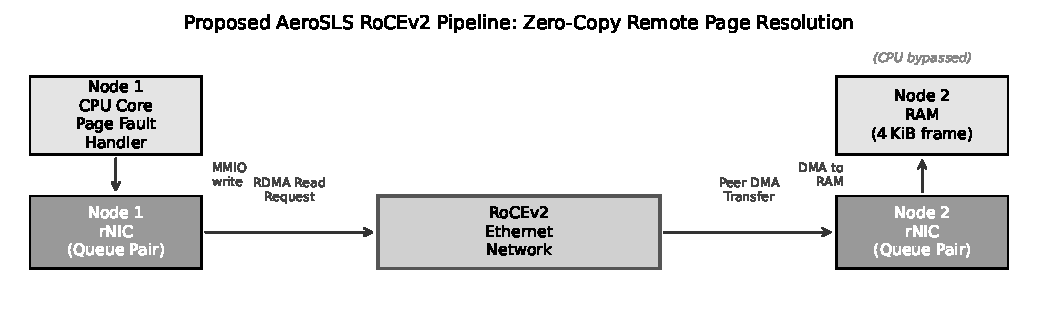
\includegraphics[width=\linewidth]{roce_pipeline.pdf}
\caption{Proposed AeroSLS zero-copy RoCEv2 integration pipeline
  for sub-microsecond distributed page resolution.}
\label{fig:roce_pipeline}
\end{figure}

When a remote page fault triggers, the kernel will post an RDMA
Read Request straight to the hardware rNIC PCIe lanes.  The
remote network card will pull the target $4\,\text{KiB}$ data
frame directly out of its local physical RAM pool using
peer-to-peer DMA over the wire.  This pipeline is projected to reduce
distributed memory synchronization delays to sub-microsecond
scales, approaching the latency of unified hardware memory
fabrics (Figure~\ref{fig:roce_pipeline}).

\subsection{SLS-Aware Compiler Plugins for Legacy Runtimes}
Finally, we aim to eliminate the necessity for explicit system
allocation wrappers by developing automated, compiler-level
optimization plugins for legacy programming languages (such as
C, C++, and Rust).  Interacting with the persistent object heap
via manual system call bindings shifts the burden of structural
safety checking entirely onto the application developer.

To make the single-level object-heap infrastructure entirely
seamless, we are engineering custom compiler front-end and
back-end passes using the LLVM infrastructure.  These plugins
will intercept standard language keywords (e.g., overloading the
C++ \texttt{new} operator or introducing a custom Rust attribute
macro such as \texttt{\#[persistent]}) during the Intermediate
Representation (LLVM-IR) compilation phase.  The compiler will
automatically insert offset-based \texttt{sls\_malloc} hooks,
manage relative pointer calculations within individual data
structures, and handle automatic alignment constraints at
compile time.  This allows legacy applications
to be ported into the AeroSLS environment and achieve
crash-consistent persistence without modifying their core
application logic.

% ============================================================
\bibliographystyle{ACM-Reference-Format}
\bibliography{aerosls_paper}

\end{document}
